% This version of CVPR template is provided by Ming-Ming Cheng.
% Please leave an issue if you found a bug:
% https://github.com/MCG-NKU/CVPR_Template.

\documentclass[review]{cvpr}
%\documentclass[final]{cvpr}

\usepackage{times}
\usepackage{epsfig}
\usepackage{graphicx}
\usepackage{subfigure}
\usepackage{amsmath}
\usepackage{amssymb}

% Include other packages here, before hyperref.

% If you comment hyperref and then uncomment it, you should delete
% egpaper.aux before re-running latex.  (Or just hit 'q' on the first latex
% run, let it finish, and you should be clear).
\usepackage[pagebackref=true,breaklinks=true,colorlinks,bookmarks=false]{hyperref}


\def\cvprPaperID{0001} % *** Enter the CVPR Paper ID here
\def\confYear{CVPR 2021}
%\setcounter{page}{4321} % For final version only


\begin{document}

%%%%%%%%% TITLE
\title{Lecture Node for Edge Detection}

\author{HeZe\\
Sun Yat-Sen University\\
{\tt\small heze_heze@icloud.com}
% For a paper whose authors are all at the same institution,
% omit the following lines up until the closing ``}''.
% Additional authors and addresses can be added with ``\and'',
% just like the second author.
% To save space, use either the email address or home page, not both
}

\maketitle


%%%%%%%%% ABSTRACT
\begin{abstract}
   This article first introduces some concepts related to edge detection, and then introduces four classic edge detection operators including sobel, scharr, laplace, and canny operators, and uses these four operators to process different pictures and compare them. Then summarized the advantages and disadvantages of these four methods, and finally proposed the improvement direction for the disadvantages of the canny operator.
\end{abstract}

%%%%%%%%% BODY TEXT
\section{Introduction}

This part will explain some concepts related to edge detection and some terms needed in the following algorithm, including image edge, noise, gradient, filtering and so on. However, this part will only introduce the basic concepts, and the specific algorithm and operation will be elaborated in detail in the following part.

%-------------------------------------------------------------------------
\subsection{Edge}

There is always an edge between two adjacent areas with different gray values, and the edge is the expression of discontinuous gray values.

Edge exists between target, background and region, so it is the most important basis for image segmentation. Since the edge is a sign of position and insensitive to the change of gray level, it is also an important feature of image matching.

\subsection{Edge Detection}

Edge detection is to find the edge contour of the object in the image, usually to find the collection of pixel points in the image whose pixel brightness changes dramatically, because these collection points often show the rough outline of the object. Edge detection can be regarded as a very important method of image feature extraction in the field of computer vision. Because if we can detect the outline of the object, and then carry out certain operations, we can represent the area, shape and other characteristics of the object.

In practice, the edges we get tend to fall into four categories:

\begin{itemize}
  \item Depth discontinuity : the object is in a different plane of the object
  \item The discontinuity of the surface direction : such as the two different faces of the cube
  \item The object material is different : this will lead to different light reflection coefficient
  \item Different lighting in the scene : such as the ground thrown by the tree sprout
\end{itemize}

\subsection{Noise}
Image noise refers to the unnecessary or redundant interference information existing in the image data. All kinds of factors in the image that hinder people's acceptance of its information can be called image noise. Noise in the image is often shown as some isolated pixel points or pixel blocks that cause strong visual effect. In general, the noise signal is not related to the object to be studied. It appears in the form of useless information and disrupts the observable information of the image. 

For digital image signal, noise is shown as large or small extreme values. These extreme values act on the real gray value of image pixels through addition and subtraction, causing bright and dark point interference to the image, greatly reducing the image quality, affecting the subsequent work of image restoration, segmentation, feature extraction, image recognition and so on.

%-------------------------------------------------------------------------
\subsection{Filter}
Filtering is the operation of filtering out the frequency of a particular band in the signal. It is an important measure to restrain and prevent interference. In the image processing, filtering is a kind of image preprocessing, filtering in the image processing signal in the specific band frequency filter, so as to retain the required band frequency signal, mainly in the preservation of the details of the image itself as far as possible under the condition of noise suppression of the image.

There are two main purposes of filtering:

\begin{itemize}
\item In order to meet some needs of image processing, filtering is used to eliminate the noise mixed with image digitizatin.
\item The image features are extracted by filtering, and the information carried by the image is simplified as other subsequent image processing, that is, the edge line is used to represent the information carried by the image.
\end{itemize}

\subsection{Image Gradient}

Image gradient refers to the rate of change of a pixel in the X and Y directions (compared with adjacent pixels) of an image. It is a two-dimensional vector composed of two components: the change of the X axis and the change of the Y axis.

The change in the X-axis refers to the pixel value on the right side of the current pixel (X plus 1) minus the pixel value on the left side of the current pixel (X minus 1).

Similarly, the change in the Y-axis is the pixel value below the current pixel (Y plus 1) minus the pixel value above the current pixel (Y minus 1).

These two components are calculated to form a two-dimensional vector, and the image gradient of the pixel is obtained. If we take the arctan of it, we get the gradient Angle.

In other words, the process of finding the image gradient can be realized by a convolution kernel: $[-1,0,1]$.



%------------------------------------------------------------------------
\section{Applicable scene}

In essence, edge pixel refers to the sharp change of gray level (singularity) in the local image range, and image edge is the collection of singularity in two-dimensional image. The edges of important visual information such as object shape, object boundary, location occlusion, shadow contour and surface texture are all generated in the image. Image edge is the most basic feature of image, which is the basis of image analysis and understanding. Edge detection is also important for object recognition. Because :

\begin{itemize}
  \item Human's eyes scan an unknown object by following its outline; 
  \item The edge of the image can be obtained, which greatly simplifies the image analysis;
  \item Many images do not have specific objects.The understanding of these images depends on their texture properties, and the extraction of these texture properties is extremely closely related to edge detection. 
\end{itemize}

 Therefore, edge detection is the premise of digital image analysis and processing. The merits and demerits of the detection results affect the application of image compression, computer vision and pattern recognition in the next step. Therefore, the research on edge detection has practical and theoretical significance.

%-------------------------------------------------------------------------
\subsection{The influence on image data compression}

In the research of image science, a lot of work is the processing of images and graphics, including the processing, storage and transmission of digital images. In particular, multimedia technology, computer vision and computer pattern recognition have been more and more widely used in people's lives. Its technical characteristics require information interactivity, real - time and synergy. From the status quo of image processing and data storage and transmission theory, the key technology in multimedia application is the compression and coding of graphics and image data to reduce data storage, reduce data transmission rate, to meet the requirements of image processing in all walks of life.

Image information can be compressed, because there is a large amount of redundant information in the original data, and human vision has "masking effect", so some information can be lost to a certain extent in the image transmission, so as to achieve a large compression ratio. The edge detection of the object in the image can extract the key features or contours of the object, and can represent the image with fewer bits to achieve the purpose of compression of image data.



%-------------------------------------------------------------------------
\subsection{The influence on pattern recognition}

In the field of artificial intelligence, pattern recognition can be realized well with digital image processing technology. Given a digital image containing multiple objects, the pattern recognition process mainly consists of three stages :

\begin{itemize}
  \item Image segmentation or image separation. Each object is detected and separated from the rest of the scene. 
  \item Feature extraction. An object is measured to form a set of n-dimensional features. 
  \item Classification. Outputs a decision to determine the category to which the object belongs. 
\end{itemize}

Accurate image edge detection is the basis of the above algorithm. In the digital recognition system, image edge extraction occupies an important position, it is located at the bottom of the system, and is dependent on other modules.

\section{Sobel Operator}

The sobel operator is one of the most common operator. It's very classical and easy.

It is a discrete differentiation operator, computing an approximation of the gradient of the image intensity function. At each point in the image, the result of the Sobel–Feldman operator is either the corresponding gradient vector or the norm of this vector. The Sobel–Feldman operator is based on convolving the image with a small, separable, and integer-valued filter in the horizontal and vertical directions and is therefore relatively inexpensive in terms of computations. On the other hand, the gradient approximation that it produces is relatively crude, in particular for high-frequency variations in the image.

\subsection{Formulation}

The operator uses two $3\times 3$ kernels which are convolved with the original image to calculate approximations of the derivatives – one for horizontal changes, and one for vertical. If we define A as the source image, and $G_x$ and $G_y$ are two images which at each point contain the horizontal and vertical derivative approximations respectively, the computations are as follows:

\begin{equation}
  \mathbf{G}_{x}=\left[\begin{array}{lll}+1 & 0 & -1 \\ +2 & 0 & -2 \\ +1 & 0 & -1\end{array}\right] * \mathbf{A} \quad
\end{equation}


and

\begin{equation}
  \mathbf{G}_{y}=\left[\begin{array}{ccc}+1 & +2 & +1 \\ 0 & 0 & 0 \\ -1 & -2 & -1\end{array}\right] * \mathbf{A}
\end{equation}

where $*$ here denotes the 2-dimensional signal processing convolution operation.

$\mathbf{G}_{x}$ can be written as


\begin{equation}
  \mathbf{G}_{x}=\left[\begin{array}{l}
1 \\
2 \\
1
\end{array}\right] *\left(\left[\begin{array}{lll}
+1 & 0 & -1
\end{array}\right] * \mathbf{A}\right)
\end{equation}

and 

\begin{equation}
  \mathbf{G}_{y}=\left[\begin{array}{c}
+1 \\
0 \\
-1
\end{array}\right] *\left(\left[\begin{array}{lll}
1 & 2 & 1
\end{array}\right] * \mathbf{A}\right)
\end{equation}



The $x$-coordinate is defined here as increasing in the right-direction, and the $y$ -coordinate is defined as increasing in the down-direction. At each point in the image, the resulting gradient approximations can be combined to give the gradient magnitude, using:

\begin{equation}
  \mathbf{G}=\sqrt{\mathbf{G}_{x}^{2}+\mathbf{G}_{y}^{2}}
\end{equation}

Using this information, we can also calculate the gradient's direction:

\begin{equation}
  \boldsymbol{\Theta}=\arctan \frac{\mathbf{G}_{y}}{\mathbf{G}_{x}}
\end{equation}


where, for example, $\boldsymbol{\theta}$ is 0 for a vertical edge which is lighter on the right side.

\subsection{Advantages}
Because Sobel operator combines Gaussian smoothing and differentiation, the result will be more anti-noise, and it has a better effect on grayscale gradient and image processing with more noise.

\subsection{Disadvantages}
Sobel operator uses intensity values only in a 3×3 region around each image point to approximate the corresponding image gradient, and it uses only integer values for the coefficients which weight the image intensities to produce the gradient approximation. In addition, when the edge of the image is more than one pixel, the Sobel operator is not very accurate in locating the edge. So the Sobel-Feldman operator represents a rather inaccurate approximation of the image gradient. 

\subsection{Scharr Operator}

As mentioned above, although Sobel operator can effectively extract image edges, it has a poor effect on weak edges in the image. Therefore, in order to extract weak edges effectively, the gap between pixel values needs to be increased, so Scharr operator is introduced.

Scharr operator is an enhancement of the difference of Sobel operator, so they have the same principle and way of using in image edge detection. The difference between the pixel values can be increased by amplifying the weight coefficients in the filter, which is the idea of the Scharr operator, it's formulation is :

\begin{equation}
  \mathbf{G}_{x}=\left[\begin{array}{lll}-3 & 0 & +3 \\ -10 & 0 & +10 \\ -3 & 0 & +3\end{array}\right] * \mathbf{A} \quad
\end{equation}


and \\

\begin{equation}
  \mathbf{G}_{y}=\left[\begin{array}{ccc}-3 & -10 & -3 \\ 0 & 0 & 0 \\ +3 & +10 & +3\end{array}\right] * \mathbf{A}
\end{equation}


The Scharr operator is just as fast as the Sobel function, but the result is much more accurate.

\section{Laplace Operator}

As one of edge detection, Laplace operator, like Sobel operator, is also an integral transformation commonly used in engineering mathematics and belongs to spatial sharpening filtering operation. The Sobel Operator calculates a first-order differential, while the Laplace Operator is a second-order differential Operator in n-dimensional Euclidean space, defined as the divergence of a gradient.

\subsection{Formulation}
Laplace operator is the simplest isotropic differential operator, which has rotation invariance. The Laplace transform of a two-dimensional graph function is the second derivative of an isotropic graph. 

Defined as:

\begin{equation}
  \text { Laplace }(f)=\frac{\partial^{2} f}{\partial x^{2}}+\frac{\partial^{2} f}{\partial y^{2}}
\end{equation}


The derivative of the discrete function degenerates into a difference, and the one-dimensional first-order difference formula is as follows:

\begin{equation}
  \frac{\partial f}{\partial x}=f^{\prime}(x)=f(x+1)-f(x)
\end{equation}


Then, the second-order difference formula can be obtained:

\begin{equation}
  \begin{array}{l}
\frac{\partial^{2} f}{\partial x^{2}}=f^{\prime \prime}(x) \approx f^{\prime}(x)-f^{\prime}(x-1) \\ \\
=f(x+1)+f(x-1)-2 f(x)
\end{array}
\end{equation}


The Laplace operator of discrete functions is obtained by differentiating the second derivatives of the Laplace operator in $x$ and $y$ directions respectively. In a two-dimensional function $f(x,y)$, the second difference of $x$ and $y$ directions are respectively:


\begin{equation}
  \begin{array}{l}
\frac{\partial^{2} f}{\partial x^{2}}=f(x+1, y)+f(x-1, y)-2 f(x, y) \\ \\
\frac{\partial^{2} f}{\partial y^{2}}=f(x, y+1)+f(x, y-1)-2 f(x, y)
\end{array}
\end{equation}


Therefore, the difference form of Laplace operator can be obtained:

\begin{equation}
\begin{split}
	  \nabla^{2}f(x, y)=&f(x+1, y)+f(x-1, y)+\\
&f(x, y+1)+f(x,y-1)-4f(x, y)
\end{split}
\end{equation}


The filter mask is written as follows:

$$\mathbf{G}=\left[\begin{array}{lll}0 & 1 & 0 \\ 1 & -4 & 1 \\ 0 & 1 & 0\end{array}\right]\quad$$

The feature of the mask is that the results of the mask are the same in the directions of 90 degrees, up, down, left and right, that is to say, there is no direction in the direction of 90 degrees. In order to make the mask also have this property in the direction of 45 degrees, the filter mask was extended and defined as:

$$\mathbf{G}=\left[\begin{array}{lll}1 & 1 & 1 \\ 1 & -8 & 1 \\ 1 & 1 & 1\end{array}\right]\quad$$

When the Laplace operator is written as a Filter Mask, its operation is similar to other spatial filtering operations. Move the Filter Mask line by line on the original image, then multiply the values in the mask by the overlapping pixels and sum them, assign the overlapping pixels in the center of the mask, assign zero to the pixels in the first and last rows and columns of the image that cannot do the above operation, and get the result of Laplace operation.

\subsection{Evaluation}

This is a second-order differential operator, which is isotropic, that is, independent of the direction of the coordinate axis, and the gradient remains the same after the rotation of the coordinate axis. However, it is sensitive to noise.

Laplacian operator is generally not used for edge detection in its original form because, as a second derivative, Laplacian operator is unacceptably sensitive to noise. At the same time, its amplitude produces calculating edge, which is undesirable for complex segmentation. Finally, the Laplacian operator cannot detect the direction of the edge. So the roles that Laplacian plays in segmentation include:

\begin{itemize}
  \item Using its zero-crossing property to locate the edge.
  \item Determine whether a pixel is on the dark side or the light side of an edge.
\end{itemize}

Generally, the Laplacian of a Gaussian (LoG) operator is used. Since the second derivative is a linear operation, the Laplacian of an image convolved by LoG is the same as the Laplacian of the image convolved by Gaussian smoothing function in the first place and then calculated. So the purpose of using the Gaussian function in the LoG formula is to smooth the image, and the purpose of using the Laplacian operator is to provide an image with zero crossover to determine the edge position. The smoothing of the image reduces the impact of noise and its main function is to offset the gradually increasing noise effect caused by the second derivative of Laplacian operator.

\section{Canny Operator}
Canny edge detection operator is a multilevel edge detection algorithm developed by John F.Canny in 1986. More importantly, Canny has created Computational Theory Ofedge Detection, which explains how the technology works. Canny edge detection algorithm is named after Canny, which is praised by many people as the best edge detection algorithm today.

The goal of Canny operator is to find an optimal edge detection algorithm. There are three main evaluation criteria for optimal edge detection:
\begin{itemize}
  \item Low error rate: Edge detection with a low error rate means that as many edges in the image as possible need to be captured accurately.
  \item High positioning: The detected edge should be precisely located at the center of the true edge.
  \item Minimum response: A given edge in the image should be marked only once and, where possible, the noise of the image should not produce false edges.
\end{itemize}

\subsection{Procedure}
Canny operator is mainly divided into the following four steps:
\begin{itemize}
  \item Eliminate noise
  \item Calculate gradient and direction angle
  \item Non-maximum suppression
  \item Use dual thresholds for edge connections
\end{itemize}

\subsubsection{Noise elimination}

Edge detection is susceptible to noisy images. Therefore, denoising is usually required before edge detection. In general, Gaussian filtering is used to remove noise, as follows: a Gaussian filter kernel of size $(2k+1)\times(2k+1)$ :

\begin{equation}
\begin{split}
	H_{i j}=\frac{1}{2 \pi \sigma^{2}} \exp (-&\frac{(i-(k+1))^{2}+(j-(k+1))^{2}}{2 \sigma^{2}}); \\ \\
	& (1 \leq i, j \leq(2 k+1))
\end{split}
\end{equation}

The size of the Gaussian convolution kernel will affect the performance of the Canny detector. The larger the size, the stronger the denoising ability, so the less noise, but the more blurred the picture, the stronger the anti-noise ability of the Canny detection algorithm, but the side effect of blurring will also lead to low positioning accuracy. In general, the size of the convolution kernel is set as $3\times 3$ or $5 \times 5$, which are shown as followed:

$$
\frac{1}{16} \times\left[\begin{array}{ccc}
1 & 2 & 1\\
2 & 4 & 2 \\
1 & 2 & 1\\
\end{array}\right]
$$

or

$$
\frac{1}{273} \times\left[\begin{array}{ccccc}
1 & 4 & 7 & 4 & 1 \\
4 & 16 & 26 & 16 & 4 \\
7 & 26 & 41 & 26 & 7 \\
4 & 16 & 26 & 16 & 4 \\
1 & 4 & 7 & 4 & 1
\end{array}\right]
$$

\subsubsection{Calculate gradient and direction angle}
The most important feature of the edge is that the gray value changes dramatically. If the gray value is regarded as the value of a binary function, then the change of the gray value can be described by the gradient of the binary function. Since the image is discrete data, the derivative can be expressed by the difference value. Difference is the gray difference in actual engineering, in short, the difference value of two pixels. A pixel has 8 neighborhoods, so it is divided into upper, lower, left and right diagonal angles. Therefore, Canny algorithm uses four operators to detect horizontal, vertical and diagonal edges in the image.

Here we can use the sobel operator which is mentioned before:

\begin{equation}
  \mathbf{G}_{x}=\left[\begin{array}{l}
1 \\
2 \\
1
\end{array}\right] *\left(\left[\begin{array}{lll}
+1 & 0 & -1
\end{array}\right] * \mathbf{A}\right)
\end{equation}

\begin{equation}
  \mathbf{G}_{y}=\left[\begin{array}{c}
+1 \\
0 \\
-1
\end{array}\right] *\left(\left[\begin{array}{lll}
1 & 2 & 1
\end{array}\right] * \mathbf{A}\right)
\end{equation}

\begin{equation}
  \mathbf{G}=\sqrt{\mathbf{G}_{x}^{2}+\mathbf{G}_{y}^{2}}
\end{equation}

\begin{equation}
  \boldsymbol{\Theta}=\arctan \frac{\mathbf{G}_{y}}{\mathbf{G}_{x}}
\end{equation}

The gradient direction is generally always perpendicular to the boundary and is grouped into four categories: vertical, horizontal, and two diagonals (i.e., $0^\circ$, $45^\circ$, $90^\circ$, and $135^\circ$).

\subsubsection{Non-maximum suppression}

The gradient image obtained from the previous step has many problems, such as edge width, weak edge interference, etc. The larger the element value in the image gradient amplitude matrix, the larger the gradient value of the point in the image, but it does not mean that the point is an edge (this is just a process of image enhancement). In Canny algorithm, non-maximum suppression is an important step in edge detection. In a general sense, it refers to looking for the local maximum value of pixel points and setting the gray value corresponding to the non-maximum point to 0, which can eliminate a large number of non-edge points.

\begin{figure}[htbp]
\centering
  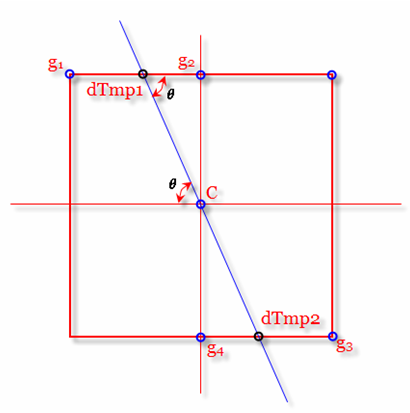
\includegraphics[scale=0.5]{../../figure/1.png}
  \caption{Non-maximum suppression principle}
  \label{fig1}
\end{figure}

As shown in Figure \ref{fig1}, to carry out non-maximum suppression, it is necessary to first determine whether the gray value of pixel point C is the maximum in its 8-value neighborhood. The direction of the blue line in Figure 1 is the gradient direction of point C, so it can be determined that its local maximum value must be distributed on this line. In other words, outside point C, the intersection points of the gradient direction, dTmp1 and dTmp2, may also be the local maximum value. Therefore, judging the grayscale of point C and the grayscale of these two points can determine whether point C is the local maximum grayscale point in its neighborhood. If it is judged that the gray value of point C is less than either of these two points, then it means that point C is not a local maximum value, and then point C can be excluded as the edge. This is how non-maximum suppression works.

In addition, I think there are two points that need to be noted:

\begin{itemize}
  \item In order to determine whether the current gradient value is a local maximum in the gradient direction, the gradient value at the current position needs to be compared with the gradient value on both sides of the gradient direction.
  \item The gradient direction should be perpendicular to the edge direction.
\end{itemize}

However, in fact, we can only get the values of 8 points in the neighborhood of point C, and dTmp1 and dTmp2 are not among them. In order to get these two values, we need to interpolate the known grays at both ends of these two points linearly, that is, interpolate dTmp1 according to G1 and G2 in Figure 1, and interpolate dTmp2 according to G3 and G4. This requires its gradient direction, which is the reason why the gradient direction matrix's $\theta$ is required to be solved in Canny algorithm above.

\subsubsection{Use dual thresholds for edge connections}
The edge quality obtained after the above three steps is already very high, but there are still many false edges. Therefore, the algorithm used in Canny algorithm is the double threshold method, and the specific idea is to select two thresholds:

\begin{itemize}
  \item If the amplitude of a pixel position exceeds a high threshold, the pixel is retained as an edge pixel.
  \item If the amplitude of a pixel position is less than the low threshold, the pixel is excluded.
  \item If the amplitude of a pixel position is between two thresholds, the pixel is reserved only if it is connected to a pixel above the high threshold.
\end{itemize}

According to the high threshold image, edges are linked into contours. When the end of the contour is reached, the algorithm will look for the point that meets the low threshold in the 8 neighborhood points of the breakpoint, and then collect new edges according to this point, until the whole image is closed.

\section{Experiment}
The above operators are used to carry out edge detection on different images, and finally compare several result images.
\subsection{Experimental Setup}
I selected two images to test various operators, of which the first image Figure \ref{og1} had lower contrast and sharpness, while the second image Figure \ref{og2} had higher contrast.

\begin{figure}[htbp]
\centering
  \includegraphics[width=3.3in]{../../figure/test1.JPG}
  \caption{Origin figure 1 for testing}
  \label{og1}
\end{figure}

\begin{figure}[htbp]
\centering
  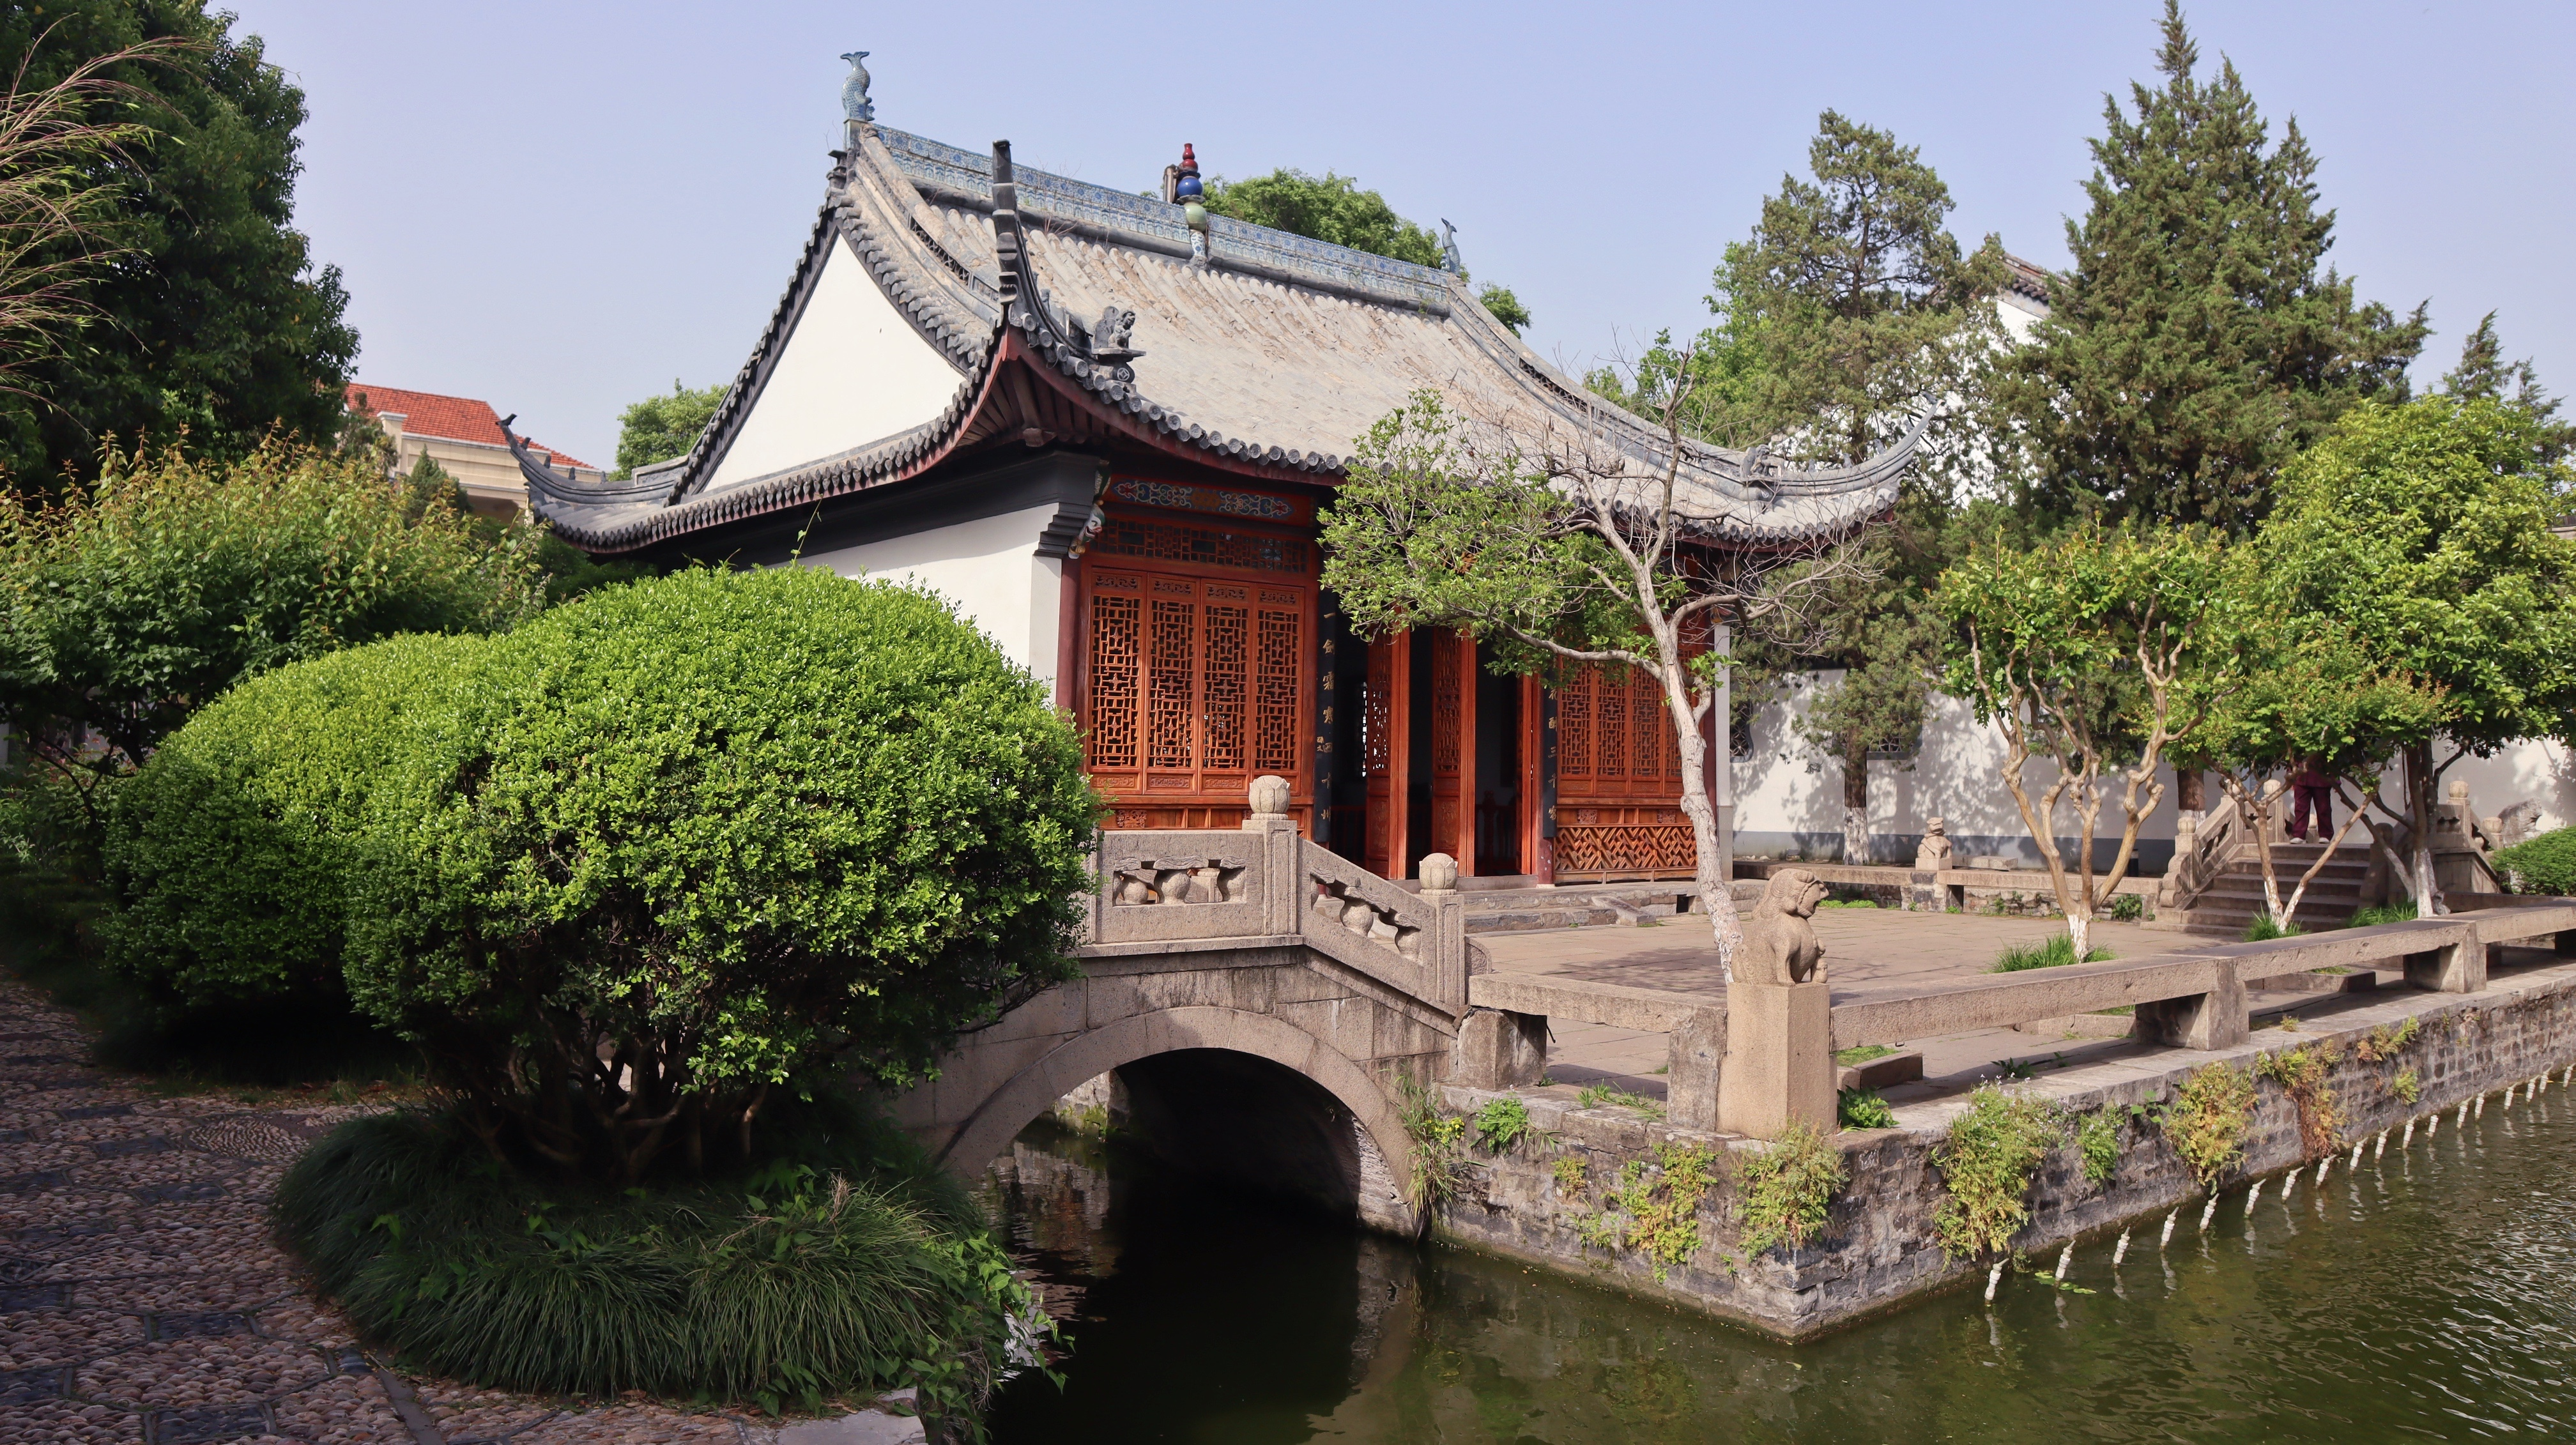
\includegraphics[width=3.3in]{../../figure/test2.JPG}
  \caption{Origin figure 2 for testing}
  \label{og2}
\end{figure}

\subsection{Sobel Operator}

The result of edge detection for these two images using Sobel operator is shown in Figure \ref{sobel}.


\begin{figure}[htbp]
\centering
  \includegraphics[width=3in]{../../figure/sobel.png}
  \caption{The result of sobel operator}
  \label{sobel}
\end{figure}

You can see that the second image is well processed, but the edges of the first image are not obvious.

\subsection{Scharr Operator}

The result of edge detection for these two images using Scharr operator is shown in Figure \ref{scharr}.

\begin{figure}[htbp]
\centering
  \includegraphics[width=3in]{../../figure/scharr.png}
  \caption{The result of scharr operator}
  \label{scharr}
\end{figure}

As an enhanced version of Sobel operator, the processing of the first graph of Scharr operator has made great progress, and the edge is clear and definite. However, the edge of the second graph is too obvious, leading to some fuzzy and unclear edges.

\subsection{Laplace Operator}

The result of edge detection for these two images using laplace operator is shown in Figure \ref{laplace}.

\begin{figure}[htbp]
\centering
  \includegraphics[width=3in]{../../figure/laplace.png}
  \caption{The result of laplace operator}
  \label{laplace}
\end{figure}

Compared with the first two, the results of the second image of Laplace operator are the best, but the first image is the worst, indicating that it is more suitable for processing images with large contrast and clear edges.

\subsection{Canny Operator}

The result of edge detection for these two images using canny operator is shown in Figure \ref{canny}.

\begin{figure}[htbp]
\centering
  \includegraphics[width=3in]{../../figure/canny.png}
  \caption{The result of canny operator}
  \label{canny}
\end{figure}

It can be seen that Canny's processing of the second image is optimal, but the outline of the first image is still too shallow, which is not as good as Scharr operator.

\section{Conclusions}
As can be seen from the above results, for images with high contrast, sharpness and obvious edge lines, Canny operator is the best. But for images with low contrast and not obvious object contour, Scharr operator is the best.

In conclusion, in actual image segmentation, only the first-order and second-order derivatives are often used. Although, in principle, higher-order derivatives can be used, but due to the influence of noise, there will be a pair of purely second-order derivatives. The sensitive phenomenon of noise, the derivative information above the third order often loses its application value. The second derivative can also explain the type of gray scale mutation. In some cases, such as an image with uniform gray scale changes, the boundary may not be found using only the first derivative, and the second derivative can provide useful information. The second derivative is also more sensitive to noise. The solution is to smooth and filter the image first to eliminate part of the noise, and then perform edge detection. However, the algorithm using the second-order derivative information is based on zero-crossing detection, so the number of edge points obtained is relatively small, which is conducive to subsequent processing and recognition work.

For the sobel operator to obtain the first derivative, because it is in the form of a filter operator, it is used to extract the edge and can use the fast convolution function, which is simple and effective, so it is widely used. The fly in the ointment is that the Sobel operator does not strictly distinguish the main body of the image from the background. In other words, the Sobel operator does not process the image based on the gray level. Because the Sobel operator does not strictly simulate the human visual and physiological characteristics, the extracted The image contour is sometimes unsatisfactory.

As for the Laplace operator for obtaining the second derivative, it is unacceptably sensitive to noise, and its amplitude produces an edge. This is an undesirable result of complex segmentation. In addition, the Laplacian operator cannot detect the direction of the edge.

The canny operator is a complete edge detection algorithm with strong anti-noise ability. It uses Gaussian filtering to smooth the image, uses the first-order partial derivative of the finite difference to calculate the gradient magnitude and direction, and suppresses the gradient magnitude. , Adopt double threshold to detect and connect edges. The advantage is that two different thresholds are used to detect strong edges and weak edges respectively, and only when the weak edges and strong edges are connected, the weak edges are included in the output image. But it has poor processing results for pictures with low contrast.

\section{Improvement and Future Work}

The reason for the poor processing of the first image of the Canny operator is probably that the Gaussian blur in the first step will also smooth the edges while removing noise, which will weaken the edge information, which may cause some needed edges to be missed in the subsequent steps. Especially weak edges and isolated edges, may be eliminated in the double threshold and connectivity calculations. It is naturally foreseeable that if the radius of the Gaussian blur is increased, the smoothing of the noise will be increased, but it will also significantly reduce the edges in the resulting edge map. Therefore, how to accurately select the Gaussian radius is the next step to continue research and optimization issues.


\begin{thebibliography}{99}  
\bibitem{ref1}John Canny, A Computational Approach to Edge Detection, IEEE Transactions on Pattern Analysis and Machine Intelligence(Volume:PAMI-8, Issue:6, Nov.1986), 1986: 1939-3539.   
\end{thebibliography}

\end{document}
